% Created 2020-06-25 qui 14:40
% Intended LaTeX compiler: pdflatex
\documentclass[11pt]{article}
\usepackage[utf8]{inputenc}
\usepackage[T1]{fontenc}
\usepackage{graphicx}
\usepackage{grffile}
\usepackage{longtable}
\usepackage{wrapfig}
\usepackage{rotating}
\usepackage[normalem]{ulem}
\usepackage{amsmath}
\usepackage{textcomp}
\usepackage{amssymb}
\usepackage{capt-of}
\usepackage{hyperref}
\usepackage[margin=0.5in]{geometry}
\author{Lucas Pereira}
\date{\today}
\title{}
\hypersetup{
 pdfauthor={Lucas Pereira},
 pdftitle={},
 pdfkeywords={},
 pdfsubject={},
 pdfcreator={Emacs 26.3 (Org mode 9.1.9)}, 
 pdflang={English}}
\begin{document}

\tableofcontents


\section{MONETDB Internals}
\label{sec:org28ecd8e}

\url{http://sites.computer.org/debull/A12mar/monetdb.pdf}
\href{https://www.monetdb.org/Documentation/MonetDBInternals/Overview}{MonetDB Internals}
\href{https://www.monetdb.org/Developers/SourceCompile}{Source Compile}

\subsection{Redesign considerations.}
\label{sec:orgae98017}
Redesign of the MonetDB software driven by the need to reduce the effort to extend the system into novel directions and to reduce
the \textbf{Total Execution Cost (TEC)}.

\textbf{TEC}:
\begin{itemize}
\item API message handling                (\textbf{A})
\item Parsing and semantic analysis       (\textbf{P})
\item Optimization and plan generation    (\textbf{O})
\item Data access to the persistent store (\textbf{D})
\item Execution of the query terms        (\textbf{E})
\item Result delivery to the application  (\textbf{R})
\end{itemize}

OLTP -> Online Transaction Processing -> expected most of the cost to be in (P,O)
OLAP -> Online Analytical Processing  -> expected most of the cost to be in (D,E,R)

\subsection{Storage Model}
\label{sec:org7b010c7}
\begin{itemize}
\item Represents relational tables using vertical fragmentation.
\item Stores each column in a separate \{(OID,value)\} table,  called a \textbf{BAT (Binary Association Table)}
\item Relies on a low-level relational algebra called the BAT algebra, which takes BATs and scalar values as input.
\item The complete result is always stored in (intermediate) BATs, and the result of an SQL query is a collection of BATs.

\item \textbf{BAT} is implemented as an ordinary C-array. OID maps to the index in the array.
\item Persistent version of \textbf{BAT} is a \textbf{memory mapped file}.
\item \textbf{O(1) positional database lookup mechanism} (MMU - memory management unit)
\end{itemize}

\subsection{All (relational) operators exploit a small set of properties:}
\label{sec:orgc82d216}
\begin{itemize}
\item seq       - the sequence base, a mapping from array index 0 into a OID value
\item key       - the values in the column are unique
\item nil       - there is at least one NIL value
\item nonil     - it is unknown if there NIL values
\item dense     - the numeric values in the column form a dense sequence
\item sorted    - the column contains a sorted list for ordered domains
\item revsorted - the column contains a reversed sorted list
\end{itemize}

\subsection{Execution Model}
\label{sec:org09504dd}
\begin{itemize}
\item \textbf{MonetDB} kernel is an abstract machine, programmed in the \textbf{MonetDB Assemblee Language (MAL)}.
\item Each relational algebra operator corresponds to a \textbf{MAL instruction} (zero degrees of freedom).
\item Each \textbf{BAT algebra operator} maps to a simple \textbf{MAL instruction}.
\end{itemize}

\subsection{Software Stack}
\label{sec:orgaad1103}
Three software layers:
\begin{itemize}
\item \textbf{FRONT-END} \textbf{Query language parser and a heuristic, language - and data model - specific optimizer}. \textbf{OUTPUT} -> logical plan expressed in MAL.
\item \textbf{BACK-END} \textbf{Collection of optimizer modules} -> assembled into an optimization pipeline
\item \textbf{MAL interpreter} -> contains the library of highly optimized implementation of the binary relational algebra operators.
\end{itemize}


\section{Binary Association Tables}
\label{sec:org5c0294f}
\begin{figure}[htbp]
\centering
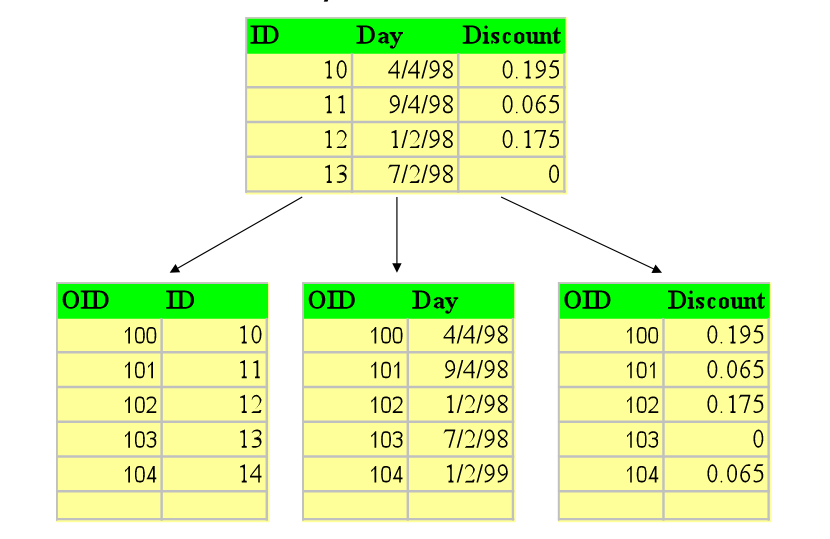
\includegraphics[width=4.0in]{./Pictures/BAT.png}
\caption{\label{fig:org957153d}
Bat Sample}
\end{figure}


\section{MAL Reference (MonetDB Assembly Language)}
\label{sec:org1e1bbd2}

\begin{itemize}
\item MAL program is considered a specification of intended computation and data flow behavior.
\item Language syntax uses a functional style definition of actions and mark those that affect the flow explicitly.
\end{itemize}

\subsection{Literals (follow the lexical conventions of C)}
\label{sec:org6cc5abb}

\begin{center}
\begin{tabular}{lll}
\hline
\textbf{Hardwire Types} & \textbf{Temporal Types} & \textbf{IPv4 addresses and URLs}\\
\hline
bit (bit) & date & inet\\
\hline
bte (byte) & daytime & url\\
\hline
chr (char) & time & UUID\\
\hline
wrd (word) & timestamp & json\\
\hline
sht (short) & - & -\\
\hline
int (integer) & - & -\\
\hline
lng (long) & - & -\\
\hline
oid (object id) & - & -\\
\hline
flt (float) & - & -\\
\hline
dbl (double) & - & -\\
\hline
str (string) & - & -\\
\hline
\end{tabular}
\end{center}

\subsection{Variables}
\label{sec:org6265c4a}

\textbf{User Defined} -> start with a letter
\textbf{Temporary}    -> start with X\_ (generated internally by optimizers)

\subsection{Instructions}
\label{sec:org823cf8d}

\textbf{One liners}   -> easy to parse

\begin{figure}[htbp]
\centering
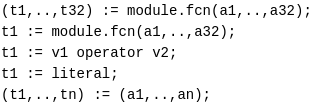
\includegraphics[width=4.0in]{./Pictures/instructions-ex.png}
\caption{\label{fig:orgf0444ea}
Instructions example}
\end{figure}

\subsection{Type System}
\label{sec:org959fffa}

\textbf{Strongly typed language}

\begin{figure}[htbp]
\centering
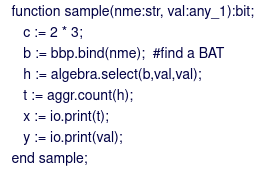
\includegraphics[width=4.0in]{./Pictures/poly-ex.png}
\caption{\label{fig:orgfac603f}
Polymophism example}
\end{figure}

\begin{itemize}
\item Polymorphic given by "any".
\item Type checker (intelligent type resolution).
\end{itemize}

\subsection{Flow of Control}
\label{sec:org2f14421}

\textbf{For statement implementation:}
\begin{figure}[htbp]
\centering
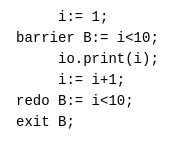
\includegraphics[width=4.0in]{./Pictures/for-ex.png}
\caption{\label{fig:orgcde0b29}
For example}
\end{figure}

\textbf{If statement implementation:}
\begin{figure}[htbp]
\centering
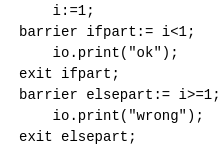
\includegraphics[width=4.0in]{./Pictures/if-ex.png}
\caption{\label{fig:org210eeaf}
If example}
\end{figure}

\subsection{Exceptions}
\label{sec:orgd9945ad}

(\textbf{To explore.})

\subsection{Functions}
\label{sec:orgb518795}

\textbf{Function example}
\begin{figure}[htbp]
\centering
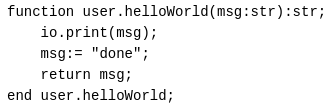
\includegraphics[width=4.0in]{./Pictures/fun-ex.png}
\caption{\label{fig:org47266f3}
Function example}
\end{figure}

\textbf{Side Effects}
\begin{itemize}
\item Functions can be pre-pended with the keyword unsafe.
\item Designates that execution of the function may change the state of the database or sends information to the client.
\item Unsafe functions are critical for the optimizers -> order of execution should be guaranteed.
\item Functions that return \textbf{:void} -> unsafe by default.
\end{itemize}

\textbf{Inline Functions}
\begin{itemize}
\item Functions prepended with the keyword \textbf{inline} are a target for the optimizers to be inlined. -> reduce the function call overhead.
\end{itemize}

\subsection{MAL Syntax}
\label{sec:org8bc6049}

\textbf{Expressed in extended Backus–Naur form (EBNF)} \href{https://en.wikipedia.org/wiki/Extended\_Backus\%E2\%80\%93Naur\_form}{Wiki}

\begin{center}
\begin{tabular}{ll}
\hline
Alternative constructors & (vertical bar) grouped by ()\\
\hline
Repetition & '+'-> at least once; '*'-> many\\
\hline
Lexical tokens & small capitals\\
\hline
\end{tabular}
\end{center}

\begin{figure}[htbp]
\centering
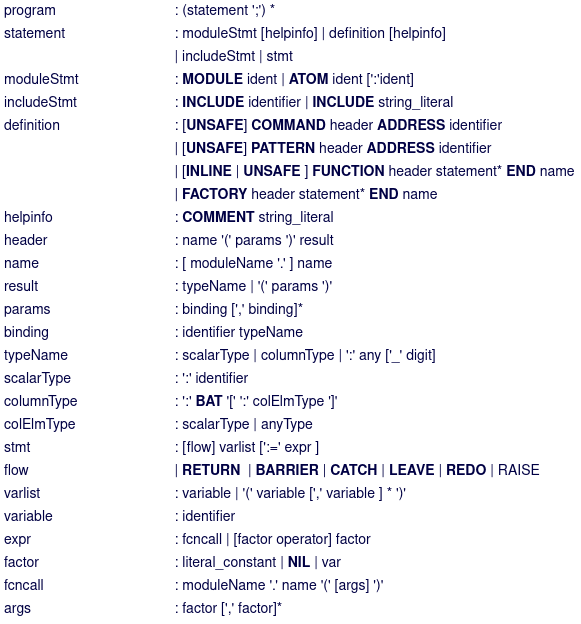
\includegraphics[width=4.0in]{./Pictures/syntax.png}
\caption{\label{fig:orgbfc69c6}
Syntax example}
\end{figure}

\subsection{MAL Interpreter}
\label{sec:org82709fd}

(\textbf{To explore.})

\subsection{MAL Debugger}
\label{sec:org07787af}

(\textbf{To explore.})

\subsection{MAL Profiler}
\label{sec:org3949670}

(\textbf{To explore.})

\subsection{MAL Optimizers}
\label{sec:orgf2a29dd}
\textbf{Triggered by experimentation and curiousity}

\begin{itemize}
\item Alias Removal
\item Building Blocks -> there are examples for a user to build a Optimizer
\item Coercions
Removes coercions that are not needed --> v:= calc.int(23);
(sloppy code-generator or function call resolution decision)

\item Common Subexpressions
\begin{figure}[htbp]
\centering
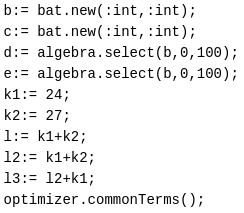
\includegraphics[width=4.0in]{./Pictures/opt-common-subs-1.png}
\caption{\label{fig:org96b654f}
Syntax example}
\end{figure}              \begin{figure}[htbp]
\centering
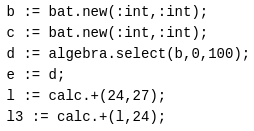
\includegraphics[width=4.0in]{./Pictures/opt-common-subs-1+.png}
\caption{\label{fig:org96b654f}
Syntax example}
\end{figure}

\item Constant Expression Evaluation

\begin{center}
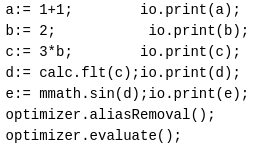
\includegraphics[width=.9\linewidth]{./Pictures/const-exps-eval-1.png}
\end{center}              \begin{center}
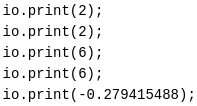
\includegraphics[width=.9\linewidth]{./Pictures/const-exps-eval-1+.png}
\end{center}

\item Cost Model
\item Data Flow
Query executions without side effects can be rearranged.
\item Garbage Collector
\item Join Paths
Looks up the MAL query and "composes" multiple joins. \textbf{algebra.join -> algebra.joinPath}
\item Landscape
\item Lifespans
\item Macro Processing
\item Memoization
\item Multiplex Functions
\item Remove Actions
\item Stack Reduction
\end{itemize}

\subsection{MAL Modules}
\label{sec:org4e6ddc2}
\begin{itemize}
\item Alarm
\item Algebra (Important)
\item BAT (Important)
\item BAT Extensions (Important)
\item BBP
\item Calculator
\item Clients (Important)
\item Debugger (Important)
\item Factories
\item Groups (Important)
\item I/O
\item Imprints
\item Inspect
\item Iterators
\item Language Extension
\item Logger
\item MAPI Interface (Important)
\item Manual
\item PCRE Library
\item Profiler
\item Remote
\item Transaction
\end{itemize}


\section{MAL Algebra}
\label{sec:org29da744}

\begin{center}
\begin{tabular}{lllll}
\hline
Operation & MAL Cmd & C Cmd & Arguments/Return & Comment\\
\hline
GroupBy & groupby & ALGgroupby & gids :: bat-columntype:oid & Produces a new BAT with groups\\
 &  &  & cnts :: bat-columntype:oid & indentified by the head column.\\
 &  &  &  & (The result contains tail times\\
 &  &  & return :: bat-columntype:oid & the head value, ie the tail\\
 &  &  &  & contains the result group sizes.)\\
\hline
Find & find & ALGfind & b :: bat-columntype:any-1 & Returns the index position of a\\
 &  &  & t :: any-1 & value. If no such BUN exists\\
 &  &  &  & return OID-nil.\\
 &  &  & return :: oid & \\
\hline
Fetch & fetch & ALGfetchoid & b :: bat-columntype:any-1 & Returns the value of the BUN at\\
 &  &  & x :: oid & x-th position with\\
 &  &  &  & 0 <= x < b.count\\
 &  &  & return :: any-1 & \\
\hline
Project & project & ALGprojecttail & b :: bat-columntype:any-1 & Fill the tail with a constant\\
 &  &  & v :: any-3 & \\
 &  &  &  & \\
 &  &  & return :: bat-columntype:any-3 & \\
\hline
Projection & projection & ALGprojection & left :: bat-columntype:oid & Project left input onto right input.\\
 &  &  & rigth :: bat-columntype:any-3 & \\
 &  &  &  & \\
 &  &  & return :: bat-columntype:any-3 & \\
\hline
Projection2 & projection2 & ALGprojection2 & left :: bat-columntype:oid & Project left input onto right inputs\\
 &  &  & rigth1 :: bat-columntype:any-3 & which should be consecutive.\\
 &  &  & rigth2 :: bat-columntype:any-3 & \\
 &  &  &  & \\
 &  &  & return :: bat-columntype:any-3 & \\
\hline
\end{tabular}
\end{center}

\textbf{BAT copying}

\begin{center}
\begin{tabular}{lllll}
\hline
Operation & MAL Cmd & C Cmd & Arguments/Return & Comment\\
\hline
Copy & copy & ALGcopy & b :: bat-columntype:any-1 & Returns physical copy of a BAT.\\
 &  &  &  & \\
 &  &  & return :: bat-columntype:any-1 & \\
\hline
Exist & exist & ALGexist & b :: bat-columntype:any-1 & Returns whether 'val' occurs in b.\\
 &  &  &  & \\
 &  &  & return :: bit & \\
\hline
\end{tabular}
\end{center}

\textbf{select}
ALGselect1
ALGselect2
ALGselect1nil
ALGselect2nil

\textbf{thetaselect}
ALGthetaselect1
ALGthetaselect2

\textbf{selectNotNil}
ALGselectNotNil

\textbf{sort}
ALGsort11
ALGsort12
ALGsort13
ALGsort21
ALGsort22
ALGsort23
ALGsort31
ALGsort32
ALGsort33

\textbf{unique}
ALGunique2
ALGunique1

\textbf{\textbf{Join operations}}
\textbf{crossproduct}
ALGcrossproduct2

\textbf{join}
ALGjoin
ALGjoin1

\textbf{leftjoing}
ALGleftjoin
ALGleftjoin1

\textbf{outerjoin}
ALGouterjoin

\textbf{semijoin}
ALGsemijoin

\textbf{thetajoin}
ALGthetajoin

\textbf{band join}
ALGbandjoin

\textbf{rangejoin}
ALGrangejoin

\textbf{difference}
ALGdifference

\textbf{intersect}
ALGintersect

\textbf{\textbf{Projection operations}}
\textbf{firstn}
ALGfirstn
\textbf{reuse}
ALGreuse

\textbf{slice}
ALGslice\(_{\text{oid}}\)
ALGslice
ALGslice\(_{\text{int}}\)
ALGslice\(_{\text{lng}}\)
\textbf{subslice}
ALGsubslice\(_{\text{lng}}\)

\textbf{\textbf{Common BAT Aggregates}}

\textbf{count}
ALGcount\(_{\text{bat}}\)
ALGcount\(_{\text{nil}}\)
\textbf{count\(_{\text{no}}\)\(_{\text{nil}}\)}
ALGcount\(_{\text{no}}\)\(_{\text{nil}}\)

\textbf{count}
ALGcountCND\(_{\text{bat}}\)
ALGcountCND\(_{\text{nil}}\)
\textbf{count\(_{\text{no}}\)\(_{\text{nil}}\)}
ALGcountCND\(_{\text{no}}\)\(_{\text{nil}}\)


\noindent\rule{\textwidth}{0.5pt}

command select(b:bat[:any\(_{\text{1}}\)], low:any\(_{\text{1}}\), high:any\(_{\text{1}}\), li:bit, hi:bit, anti:bit) :bat[:oid]
address ALGselect1
comment "Select all head values for which the tail value is in range.
	Input is a dense-headed BAT, output is a dense-headed BAT with in
	the tail the head value of the input BAT for which the tail value
	is between the values low and high (inclusive if li respectively
	hi is set).  The output BAT is sorted on the tail value.  If low
	or high is nil, the boundary is not considered (effectively - and
\begin{itemize}
\item infinity).  If anti is set, the result is the complement.  Nil
\end{itemize}
values in the tail are never matched, unless low=nil, high=nil,
li=1, hi=1, anti=0.  All non-nil values are returned if low=nil,
high=nil, and li, hi are not both 1, or anti=1.
Note that the output is suitable as second input for the other
version of this function.";

command select(b:bat[:any\(_{\text{1}}\)], s:bat[:oid], low:any\(_{\text{1}}\), high:any\(_{\text{1}}\), li:bit, hi:bit, anti:bit) :bat[:oid]
address ALGselect2
comment "Select all head values of the first input BAT for which the tail value
	is in range and for which the head value occurs in the tail of the
	second input BAT.
	The first input is a dense-headed BAT, the second input is a
	dense-headed BAT with sorted tail, output is a dense-headed BAT
	with in the tail the head value of the input BAT for which the
	tail value is between the values low and high (inclusive if li
	respectively hi is set).  The output BAT is sorted on the tail
	value.  If low or high is nil, the boundary is not considered
	(effectively - and + infinity).  If anti is set, the result is the
	complement.  Nil values in the tail are never matched, unless
	low=nil, high=nil, li=1, hi=1, anti=0.  All non-nil values are
	returned if low=nil, high=nil, and li, hi are not both 1, or anti=1.
	Note that the output is suitable as second input for this
	function.";

command select(b:bat[:any\(_{\text{1}}\)], low:any\(_{\text{1}}\), high:any\(_{\text{1}}\), li:bit, hi:bit, anti:bit, unknown:bit) :bat[:oid]
address ALGselect1nil
comment "With unknown set, each nil != nil";

command select(b:bat[:any\(_{\text{1}}\)], s:bat[:oid], low:any\(_{\text{1}}\), high:any\(_{\text{1}}\), li:bit, hi:bit, anti:bit, unknown:bit) :bat[:oid]
address ALGselect2nil
comment "With unknown set, each nil != nil";

command thetaselect(b:bat[:any\(_{\text{1}}\)], val:any\(_{\text{1}}\), op:str) :bat[:oid]
address ALGthetaselect1
comment "Select all head values for which the tail value obeys the relation
	value OP VAL.
	Input is a dense-headed BAT, output is a dense-headed BAT with in
	the tail the head value of the input BAT for which the
	relationship holds.  The output BAT is sorted on the tail value.";

command thetaselect(b:bat[:any\(_{\text{1}}\)], s:bat[:oid], val:any\(_{\text{1}}\), op:str) :bat[:oid]
address ALGthetaselect2
comment "Select all head values of the first input BAT for which the tail value
	obeys the relation value OP VAL and for which the head value occurs in
	the tail of the second input BAT.
	Input is a dense-headed BAT, output is a dense-headed BAT with in
	the tail the head value of the input BAT for which the
	relationship holds.  The output BAT is sorted on the tail value.";


command selectNotNil(b:bat[:any\(_{\text{2}}\)]):bat[:any\(_{\text{2}}\)]
address ALGselectNotNil
comment "Select all not-nil values";

command sort(b:bat[:any\(_{\text{1}}\)], reverse:bit, nilslast:bit, stable:bit) :bat[:any\(_{\text{1}}\)]
address ALGsort11
comment "Returns a copy of the BAT sorted on tail values.
         The order is descending if the reverse bit is set.
		 This is a stable sort if the stable bit is set.";
command sort(b:bat[:any\(_{\text{1}}\)], reverse:bit, nilslast:bit, stable:bit) (:bat[:any\(_{\text{1}}\)], :bat[:oid])
address ALGsort12
comment "Returns a copy of the BAT sorted on tail values and a BAT that
         specifies how the input was reordered.
         The order is descending if the reverse bit is set.
		 This is a stable sort if the stable bit is set.";
command sort(b:bat[:any\(_{\text{1}}\)], reverse:bit, nilslast:bit, stable:bit) (:bat[:any\(_{\text{1}}\)], :bat[:oid], :bat[:oid])
address ALGsort13
comment "Returns a copy of the BAT sorted on tail values, a BAT that specifies
         how the input was reordered, and a BAT with group information.
         The order is descending if the reverse bit is set.
		 This is a stable sort if the stable bit is set.";
command sort(b:bat[:any\(_{\text{1}}\)], o:bat[:oid], reverse:bit, nilslast:bit, stable:bit) :bat[:any\(_{\text{1}}\)]
address ALGsort21
comment "Returns a copy of the BAT sorted on tail values.
         The order is descending if the reverse bit is set.
		 This is a stable sort if the stable bit is set.";
command sort(b:bat[:any\(_{\text{1}}\)], o:bat[:oid], reverse:bit, nilslast:bit, stable:bit) (:bat[:any\(_{\text{1}}\)], :bat[:oid])
address ALGsort22
comment "Returns a copy of the BAT sorted on tail values and a BAT that
         specifies how the input was reordered.
         The order is descending if the reverse bit is set.
		 This is a stable sort if the stable bit is set.";
command sort(b:bat[:any\(_{\text{1}}\)], o:bat[:oid], reverse:bit, nilslast:bit, stable:bit) (:bat[:any\(_{\text{1}}\)], :bat[:oid], :bat[:oid])
address ALGsort23
comment "Returns a copy of the BAT sorted on tail values, a BAT that specifies
         how the input was reordered, and a BAT with group information.
         The order is descending if the reverse bit is set.
		 This is a stable sort if the stable bit is set.";
command sort(b:bat[:any\(_{\text{1}}\)], o:bat[:oid], g:bat[:oid], reverse:bit, nilslast:bit, stable:bit) :bat[:any\(_{\text{1}}\)]
address ALGsort31
comment "Returns a copy of the BAT sorted on tail values.
         The order is descending if the reverse bit is set.
		 This is a stable sort if the stable bit is set.";
command sort(b:bat[:any\(_{\text{1}}\)], o:bat[:oid], g:bat[:oid], reverse:bit, nilslast:bit, stable:bit) (:bat[:any\(_{\text{1}}\)], :bat[:oid])
address ALGsort32
comment "Returns a copy of the BAT sorted on tail values and a BAT that
         specifies how the input was reordered.
         The order is descending if the reverse bit is set.
		 This is a stable sort if the stable bit is set.";
command sort(b:bat[:any\(_{\text{1}}\)], o:bat[:oid], g:bat[:oid], reverse:bit, nilslast:bit, stable:bit) (:bat[:any\(_{\text{1}}\)], :bat[:oid], :bat[:oid])
address ALGsort33
comment "Returns a copy of the BAT sorted on tail values, a BAT that specifies
         how the input was reordered, and a BAT with group information.
         The order is descending if the reverse bit is set.
		 This is a stable sort if the stable bit is set.";

command unique(b:bat[:any\(_{\text{1}}\)], s:bat[:oid]) :bat[:oid]
address ALGunique2
comment "Select all unique values from the tail of the first input.
	Input is a dense-headed BAT, the second input is a
	dense-headed BAT with sorted tail, output is a dense-headed
	BAT with in the tail the head value of the input BAT that was
	selected.  The output BAT is sorted on the tail value.  The
	second input BAT is a list of candidates.";
command unique(b:bat[:any\(_{\text{1}}\)]) :bat[:oid]
address ALGunique1
comment "Select all unique values from the tail of the input.
	Input is a dense-headed BAT, output is a dense-headed BAT with
	in the tail the head value of the input BAT that was selected.
	The output BAT is sorted on the tail value.";


command crossproduct( left:bat[:any\(_{\text{1}}\)], right:bat[:any\(_{\text{2}}\)], max\(_{\text{one}}\):bit)
		(l:bat[:oid],r:bat[:oid])
address ALGcrossproduct2
comment "Returns 2 columns with all BUNs, consisting of the head-oids
	  from 'left' and 'right' for which there are BUNs in 'left'
	  and 'right' with equal tails";

command join(l:bat[:any\(_{\text{1}}\)],r:bat[:any\(_{\text{1}}\)],sl:bat[:oid],sr:bat[:oid],nil\(_{\text{matches}}\):bit,estimate:lng) (:bat[:oid],:bat[:oid])
address ALGjoin
comment "Join";

command join(l:bat[:any\(_{\text{1}}\)],r:bat[:any\(_{\text{1}}\)],sl:bat[:oid],sr:bat[:oid],nil\(_{\text{matches}}\):bit,estimate:lng) :bat[:oid]
address ALGjoin1
comment "Join; only produce left output";

command leftjoin(l:bat[:any\(_{\text{1}}\)],r:bat[:any\(_{\text{1}}\)],sl:bat[:oid],sr:bat[:oid],nil\(_{\text{matches}}\):bit,estimate:lng) (:bat[:oid],:bat[:oid])
address ALGleftjoin
comment "Left join with candidate lists";

command leftjoin(l:bat[:any\(_{\text{1}}\)],r:bat[:any\(_{\text{1}}\)],sl:bat[:oid],sr:bat[:oid],nil\(_{\text{matches}}\):bit,estimate:lng) :bat[:oid]
address ALGleftjoin1
comment "Left join with candidate lists; only produce left output";

command outerjoin(l:bat[:any\(_{\text{1}}\)],r:bat[:any\(_{\text{1}}\)],sl:bat[:oid],sr:bat[:oid],nil\(_{\text{matches}}\):bit,estimate:lng) (:bat[:oid],:bat[:oid])
address ALGouterjoin
comment "Left outer join with candidate lists";

command semijoin(l:bat[:any\(_{\text{1}}\)],r:bat[:any\(_{\text{1}}\)],sl:bat[:oid],sr:bat[:oid],nil\(_{\text{matches}}\):bit,max\(_{\text{one}}\):bit,estimate:lng) (:bat[:oid],:bat[:oid])
address ALGsemijoin
comment "Semi join with candidate lists";

command thetajoin(l:bat[:any\(_{\text{1}}\)],r:bat[:any\(_{\text{1}}\)],sl:bat[:oid],sr:bat[:oid],op:int,nil\(_{\text{matches}}\):bit,estimate:lng) (:bat[:oid],:bat[:oid])
address ALGthetajoin
comment "Theta join with candidate lists";

command bandjoin(l:bat[:any\(_{\text{1}}\)],r:bat[:any\(_{\text{1}}\)],sl:bat[:oid],sr:bat[:oid],c1:any\(_{\text{1,c2}}\):any\(_{\text{1,li}}\):bit,hi:bit,estimate:lng) (:bat[:oid],:bat[:oid])
address ALGbandjoin
comment "Band join: values in l and r match if r - c1 <[=] l <[=] r + c2";

command rangejoin(l:bat[:any\(_{\text{1}}\)],r1:bat[:any\(_{\text{1}}\)],r2:bat[:any\(_{\text{1}}\)],sl:bat[:oid],sr:bat[:oid],li:bit,hi:bit,anti:bit,symmetric:bit,estimate:lng) (:bat[:oid],:bat[:oid])
address ALGrangejoin
comment "Range join: values in l and r1/r2 match if r1 <[=] l <[=] r2";

command difference(l:bat[:any\(_{\text{1}}\)],r:bat[:any\(_{\text{1}}\)],sl:bat[:oid],sr:bat[:oid],nil\(_{\text{matches}}\):bit,nil\(_{\text{clears}}\):bit,estimate:lng) :bat[:oid]
address ALGdifference
comment "Difference of l and r with candidate lists";

command intersect(l:bat[:any\(_{\text{1}}\)],r:bat[:any\(_{\text{1}}\)],sl:bat[:oid],sr:bat[:oid],nil\(_{\text{matches}}\):bit,max\(_{\text{one}}\):bit,estimate:lng) :bat[:oid]
address ALGintersect
comment "Intersection of l and r with candidate lists (i.e. half of semi-join)";

pattern firstn(b:bat[:any], n:lng, asc:bit, nilslast:bit, distinct:bit) :bat[:oid]
address ALGfirstn
comment "Calculate first N values of B";
pattern firstn(b:bat[:any], s:bat[:oid], n:lng, asc:bit, nilslast:bit, distinct:bit) :bat[:oid]
address ALGfirstn
comment "Calculate first N values of B with candidate list S";
pattern firstn(b:bat[:any], s:bat[:oid], g:bat[:oid], n:lng, asc:bit, nilslast:bit, distinct:bit) :bat[:oid]
address ALGfirstn
comment "Calculate first N values of B with candidate list S";
pattern firstn(b:bat[:any], n:lng, asc:bit, nilslast:bit, distinct:bit) (:bat[:oid],:bat[:oid])
address ALGfirstn
comment "Calculate first N values of B";
pattern firstn(b:bat[:any], s:bat[:oid], n:lng, asc:bit, nilslast:bit, distinct:bit) (:bat[:oid],:bat[:oid])
address ALGfirstn
comment "Calculate first N values of B with candidate list S";
pattern firstn(b:bat[:any], s:bat[:oid], g:bat[:oid], n:lng, asc:bit, nilslast:bit, distinct:bit) (:bat[:oid],:bat[:oid])
address ALGfirstn
comment "Calculate first N values of B with candidate list S";

command reuse(b:bat[:any\(_{\text{1}}\)]):bat[:any\(_{\text{1}}\)]
address ALGreuse
comment "Reuse a temporary BAT if you can. Otherwise,
	allocate enough storage to accept result of an
 	operation (not involving the heap)";

command slice(b:bat[:any\(_{\text{1}}\)], x:oid, y:oid) :bat[:any\(_{\text{1}}\)]
address ALGslice\(_{\text{oid}}\)
comment "Return the slice based on head oid x till y (exclusive).";

command slice(b:bat[:any\(_{\text{1}}\)], x:lng, y:lng) :bat[:any\(_{\text{1}}\)]
address ALGslice
comment "Return the slice with the BUNs at position x till y.";

command slice(b:bat[:any\(_{\text{1}}\)], x:int, y:int) :bat[:any\(_{\text{1}}\)]
address ALGslice\(_{\text{int}}\)
comment "Return the slice with the BUNs at position x till y.";

command slice(b:bat[:any\(_{\text{1}}\)], x:lng, y:lng) :bat[:any\(_{\text{1}}\)]
address ALGslice\(_{\text{lng}}\)
comment "Return the slice with the BUNs at position x till y.";

command subslice(b:bat[:any\(_{\text{1}}\)], x:lng, y:lng) :bat[:oid]
address ALGsubslice\(_{\text{lng}}\)
comment "Return the oids of the slice with the BUNs at position x till y.";

module aggr;

command count( b:bat[:any] ) :lng
address ALGcount\(_{\text{bat}}\)
comment "Return the current size (in number of elements) in a BAT.";
command count ( b:bat[:any], ignore\(_{\text{nils}}\):bit ) :lng
address ALGcount\(_{\text{nil}}\)
comment "Return the number of elements currently in a BAT ignores
		BUNs with nil-tail iff ignore\(_{\text{nils}}\)==TRUE.";
command count\(_{\text{no}}\)\(_{\text{nil}}\) ( b:bat[:any\(_{\text{2}}\)]) :lng
address ALGcount\(_{\text{no}}\)\(_{\text{nil}}\)
comment "Return the number of elements currently
	in a BAT ignoring BUNs with nil-tail";

command count( b:bat[:any], cnd:bat[:oid] ) :lng
address ALGcountCND\(_{\text{bat}}\)
comment "Return the current size (in number of elements) in a BAT.";
command count ( b:bat[:any], cnd:bat[:oid], ignore\(_{\text{nils}}\):bit ) :lng
address ALGcountCND\(_{\text{nil}}\)
comment "Return the number of elements currently in a BAT ignores
		BUNs with nil-tail iff ignore\(_{\text{nils}}\)==TRUE.";
command count\(_{\text{no}}\)\(_{\text{nil}}\) ( b:bat[:any\(_{\text{2}}\)], cnd:bat[:oid]) :lng
address ALGcountCND\(_{\text{no}}\)\(_{\text{nil}}\)
comment "Return the number of elements currently
	in a BAT ignoring BUNs with nil-tail";

command cardinality( b:bat[:any\(_{\text{2}}\)] ) :lng
address ALGcard
comment "Return the cardinality of the BAT tail values.";

\#SQL uses variable head types
command min(b:bat[:any\(_{\text{2}}\)]):any\(_{\text{2}}\)
address ALGminany
comment "Return the lowest tail value or nil.";

command min(b:bat[:any\(_{\text{2}}\)], skipnil:bit):any\(_{\text{2}}\)
address ALGminany\(_{\text{skipnil}}\)
comment "Return the lowest tail value or nil.";

command max(b:bat[:any\(_{\text{2}}\)]):any\(_{\text{2}}\)
address ALGmaxany
comment "Return the highest tail value or nil.";

command max(b:bat[:any\(_{\text{2}}\)], skipnil:bit):any\(_{\text{2}}\)
address ALGmaxany\(_{\text{skipnil}}\)
comment "Return the highest tail value or nil.";

pattern avg(b:bat[:any\(_{\text{2}}\)]) :dbl
address CMDcalcavg
comment "Gives the avg of all tail values";

pattern avg(b:bat[:any\(_{\text{2}}\)], scale:int) :dbl
address CMDcalcavg
comment "Gives the avg of all tail values";

command stdev(b:bat[:any\(_{\text{2}}\)]) :dbl
address ALGstdev
comment "Gives the standard deviation of all tail values";
command stdevp(b:bat[:any\(_{\text{2}}\)]) :dbl
address ALGstdevp
comment "Gives the standard deviation of all tail values";
command variance(b:bat[:any\(_{\text{2}}\)]) :dbl
address ALGvariance
comment "Gives the variance of all tail values";
command variancep(b:bat[:any\(_{\text{2}}\)]) :dbl
address ALGvariancep
comment "Gives the variance of all tail values";

command covariance(b1:bat[:any\(_{\text{2}}\)],b2:bat[:any\(_{\text{2}}\)]) :dbl
address ALGcovariance
comment "Gives the covariance of all tail values";
command covariancep(b1:bat[:any\(_{\text{2}}\)],b2:bat[:any\(_{\text{2}}\)]) :dbl
address ALGcovariancep
comment "Gives the covariance of all tail values";
command corr(b1:bat[:any\(_{\text{2}}\)],b2:bat[:any\(_{\text{2}}\)]) :dbl
address ALGcorr
comment "Gives the correlation of all tail values";
\end{document}
